\documentclass{sigchi}

% Use this command to override the default ACM copyright statement (e.g. for preprints). 
% Consult the conference website for the camera-ready copyright statement.


%% EXAMPLE BEGIN -- HOW TO OVERRIDE THE DEFAULT COPYRIGHT STRIP -- (July 22, 2013 - Paul Baumann)
% \toappear{Permission to make digital or hard copies of all or part of this work for personal or classroom use is 	granted without fee provided that copies are not made or distributed for profit or commercial advantage and that copies bear this notice and the full citation on the first page. Copyrights for components of this work owned by others than ACM must be honored. Abstracting with credit is permitted. To copy otherwise, or republish, to post on servers or to redistribute to lists, requires prior specific permission and/or a fee. Request permissions from permissions@acm.org. \\
% {\emph{CHI'14}}, April 26--May 1, 2014, Toronto, Canada. \\
% Copyright \copyright~2014 ACM ISBN/14/04...\$15.00. \\
% DOI string from ACM form confirmation}
%% EXAMPLE END -- HOW TO OVERRIDE THE DEFAULT COPYRIGHT STRIP -- (July 22, 2013 - Paul Baumann)


% Arabic page numbers for submission. 
% Remove this line to eliminate page numbers for the camera ready copy
\pagenumbering{arabic}


% Load basic packages
\usepackage{balance}  % to better equalize the last page
\usepackage{graphics} % for EPS, load graphicx instead
\usepackage{times}    % comment if you want LaTeX's default font
\usepackage{url}      % llt: nicely formatted URLs
\usepackage{array}
\usepackage{listings}
\usepackage{enumitem}
\usepackage[svgnames]{xcolor}

% llt: Define a global style for URLs, rather that the default one
\makeatletter
\def\url@leostyle{%
  \@ifundefined{selectfont}{\def\UrlFont{\sf}}{\def\UrlFont{\small\bf\ttfamily}}}
\makeatother
\urlstyle{leo}


% To make various LaTeX processors do the right thing with page size.
\def\pprw{8.5in}
\def\pprh{11in}
\special{papersize=\pprw,\pprh}
\setlength{\paperwidth}{\pprw}
\setlength{\paperheight}{\pprh}
\setlength{\pdfpagewidth}{\pprw}
\setlength{\pdfpageheight}{\pprh}

% Make sure hyperref comes last of your loaded packages, 
% to give it a fighting chance of not being over-written, 
% since its job is to redefine many LaTeX commands.
\usepackage[pdftex]{hyperref}
\hypersetup{
pdftitle={SIGCHI Conference Proceedings Format},
pdfauthor={LaTeX},
pdfkeywords={SIGCHI, proceedings, archival format},
bookmarksnumbered,
pdfstartview={FitH},
colorlinks,
citecolor=black,
filecolor=black,
linkcolor=black,
urlcolor=black,
breaklinks=true,
}

% create a shortcut to typeset table headings
\newcommand\tabhead[1]{\small\textbf{#1}}


%\newenvironment{packed_enum}{
%\begin{enumerate}
%  \setlength{\itemsep}{1pt}
%  \setlength{\parskip}{0pt}
%  \setlength{\parsep}{0pt}
%}{\end{enumerate}}
%
%
%\newenvironment{packed_itemize}{
%\begin{itemize}
%  \setlength{\itemsep}{1pt}
%  \setlength{\parskip}{0pt}
%  \setlength{\parsep}{0pt}
%}{\end{itemize}}
\usepackage{enumitem}
\setlist[enumerate]{itemsep=0mm}
\setlist[itemize]{itemsep=0mm}


\lstdefinelanguage{lil}
{ 
keywords={
actor,data,interactor,
event,flow,constant,
in,or,from,to,
on,when,trigger,after,before,until,first,current,last,value,of,
if,then,else,
true,false
},
sensitive=false,
morecomment=[l]{//},
morecomment=[s]{/*}{*/},
morestring=[b]",
}

\lstset{
    language=lil,
    basicstyle=\ttfamily\scriptsize,           % print whole listing small
    keywordstyle=\color{black}\bf\ttfamily,% underlined bold black keywords
    tabsize=2,                    % sets default tabsize to 2 spaces
    captionpos =b                 % sets the caption-position to bottom
    keepspaces = true             % keeps spaces in text
    % identifierstyle=,           % nothing happens
    commentstyle=\textit,         % white comments
    stringstyle=\ttfamily,        % typewriter type for strings
    showstringspaces=false,       % no special string spaces
    columns=flexible,             % colonnes "flexibles"
    basewidth={0.45em},           % dimension des colonnes
    fontadjust=true,              % pour ajuster les polices
    breaklines=true,              % pour le retour à la ligne dans les colonnes
	backgroundcolor=\color{gray!5!white},
	moredelim=**[is][\color{magenta}]{@m}{@m},
	moredelim=**[is][\color{blue}]{@b}{@b},
	moredelim=**[is][\color{cyan}]{@c}{@c},
	moredelim=**[is][\color{green!80!black}]{@g}{@g},
	moredelim=**[is][\color{yellow!65!black}]{@y}{@y},
	moredelim=**[is][\color{orange}]{@o}{@o},
	moredelim=**[is][\color{red}]{@r}{@r},
}


% End of preamble. Here it comes the document.
\begin{document}

\title{A formal language for critical embedded user interfaces} 

\numberofauthors{1}
\author{
  \alignauthor Vincent Lecrubier\\
    \affaddr{ONERA - DTIM}\\
    \affaddr{2 Avenue Edouard Belin}\\
    \affaddr{31400, Toulouse, France}\\
    \email{Vincent.Lecrubier@onera.fr}
 }


\maketitle

\begin{abstract}
The LIL Interaction Language (LIL) is a domain-specific language (DSL) which aims at enhancing the design process of critical user interfaces (UIs). LIL is a human-readable textual language, and has formal semantics. The ambition of LIL is to become a \textit{lingua franca} between stakeholders of the critical UI specification process. This paper describes LIL positioning amongst other similar approaches, and the main concepts of LIL. We will also present ongoing work around the LIL framework, which leverage the expressiveness of the language in order to offer tools for verification, validation and code generation.
\end{abstract}

\keywords{
	Human Machine Interface; User Interface; Design; Specification; Verification; Validation; Formal Language; Domain-Specific Language.
}

\category{H.5.2.}{User Interfaces}{Evaluation/methodology}abstr%%%%%%%%%%%%%%%%%%%%%%%%%%%%%%%%%%%%%%%%%%%%%%%%%%%%%%%%%%%%%%%%%%%%%%%%%
\section{Introduction}
Critical  embedded  UIs conception  is  a discipline  which  lies at  the  limits  of  two software  engineering domains:   embedded   software    development   and   user   interface development. As a consequence,  critical embedded user interfaces must comply with  a set  of conflicting constraints.

While  embedded software  makes robustness  a priority,  UIs  must be flexible  and  configurable.   While  embedded  systems  have  limited ressources,   UIs   must   be   complete   and   integrate   lots   of functionalities.   While   critical   software  have   strong   timing constraints, UIs  must be user friendly  and let the  user interact at his  own pace.  While critical  systems are  often real-time, UIs are mostly event-driven.

This  set  of conflicting  constraints  is  a  strong limitation  for critical  UIs, and  makes  their development  particularly costly  and time-consuming. A good critical  UI development process should take  into account the methods   and  tools   in  use   for  both   of  these   domains. 

\begin{figure}[htbp]
\begin{center}
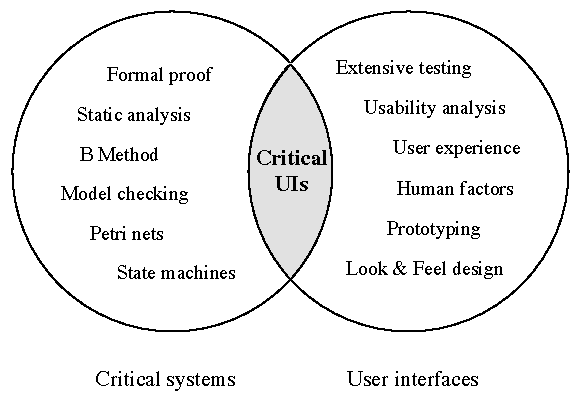
\includegraphics[width=0.8\columnwidth]{twoclashingdomains}
\caption{Two clashing domains}
\label{fig:twoclashingdomains}
\end{center}
\end{figure}

%The apparition  of model-based development  has been a big  leap ahead for non-critical UI  development, allowing for more complex  UIs to be designed in a  quicker and cheaper way. However,  critical UIs did not really  profit  yet  from  this   new  fresh  air.  They  indeed  lack development  methodologies and  tools which  would be  compatible with safety requirements while allowing quick and efficient development.


%%%%%%%%%%%%%%%%%%%%%%%%%%%%%%%%%%%%%%%%%%%%%%%%%%%%%%%%%%%%%%%%%%%%%%%%%
\section{Context}

This project  tends to  make a constructive  use of formal  methods in critical UIs development.  As so, it relies on  previous work on this subject.  Much work  was already  performed on  formal  modeling of software aspects of UIs by suggesting two main approaches. 

The first one is based on proof systems.
%where a model of the system is described by  sets of variables,  sets of operations, sets  of events, timing properties and  invariants. Operations must preserve invariants and  properties. To  ensure the  correctness of  these specifications, proof obligations are generated and must be proved. So, 
For example, Z and  VDM  were  used  to  define  atomic  structures  of  interactions (\cite{Duke-Harrison93a},\cite{Duke-Harrison93b}) and  HOL (High Order Logic Theorem  Prover) was used to check  user interface specification (\cite{Bumbulis96}).  B system was also  used for the proof of incremental specifications  (\cite{yamine98a},\cite{yamine04}).

The second one  is based on the evaluation of  logical properties on  state transition  systems. This  technique was  used, for example, to  verify formally with SMV some properties  of interactive systems    (\cite{Campos97}).    Model    checking    was   used    in (\cite{Palanque95},\cite{Navarre03}) where the user and the system are modeled by object Petri nets (ICOs). Model checking was also coupled  with static analysis of program codes in \cite{ausbourg98}  or \cite{Cortier2008} to extract  and abstract a formal model of an interactive  system and to check various properties. Modeling and analyzing of human-automation  interaction has also been demonstrated in \cite{Rushby01}, \cite{bolton2011} and \cite{combefis2012}.

Figure~\ref{fig:uimethods} describe the positioning of LIL amongst some other methods and tools currently in use or development.

\begin{figure*}[!htbp]
\begin{center}
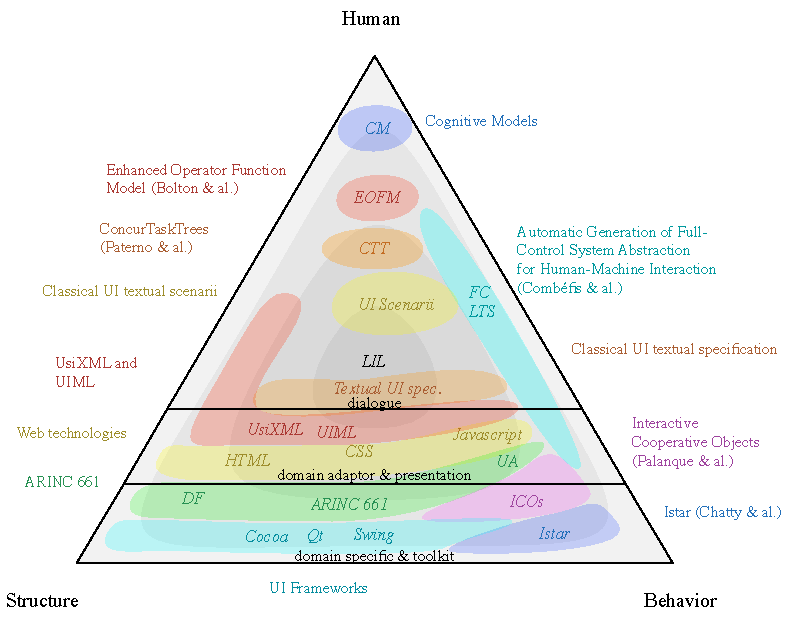
\includegraphics[width=0.6\textwidth]{uimethods.pdf}
\caption{LIL (in light grey) positioning amongst other UI development methods and tools (in colors), analyzed around 3 main axes: structural aspects, behavioral aspects and human aspects. Methods which describe an aspect with a high level of detail are found close to the edges of the figure, while higher level, more abstract methods are found closer to the center of the figure. For reference, the Arch model \protect\cite{Bass91} is represented with black frames.}
\label{fig:uimethods}
\end{center}
\end{figure*}

%%%%%%%%%%%%%%%%%%%%%%%%%%%%%%%%%%%%%%%%%%%%%%%%%%%%%%%%%%%%%%%%%%%%%%%%%
\section{Goals}

This project  aims at inverting the approach  in \cite{ausbourg98} or \cite{Cortier2008}  by  defining  a  language  which  would  allow  to formally describe and  model the behavior  of UIs.  The model perimeter is centered around the \emph{dialog controller} of the UI Arch Model from \cite{Bass91}, but allows to progressively expand the model into both sides of the Arch Model. 
%The model will be using abstractions to perform model checking on the high level behavior of UIs.

This project has similarities with the I* approach in \cite{chatty-sc-2008}. Being driven by a similar set of constraints, we share the idea that an ideal development process should rely on a unified framework which supports modularity and multiple levels of granularity. 

One of the main goals of LIL is to be useful in the earliest phases of the UI specification process, which implies a strong emphasis on abstract UI modeling as described in 
%\cite{abstractuiw3} or 
\cite{Paterno:2009:MUD:1614390.1614394}. LIL also aims at being a common language for all stakeholders related to the UI conception process, and this implies that it has a simple and clean syntax, which seems a natural conclusion to the ideas expressed in \cite{chatty2007}.

LIL promotes best practices in critical system development,
%, as seen in \cite{bestpracticecriticalsystems}, 
such as Modularity, Reusability, Error propagation prevention, Bottleneck identification and Traceability.
%\begin{itemize}
%\item \textit{Modularity} and \textit{Reusability} are enforced through the hierarchical structure of interactors that LIL imposes, unlike many other UI frameworks such as \cite{Branton:2013:TRI:2494603.2480312}, which are not designed specifically for critical UIs.
%\item \textit{Error propagation prevention} is enhanced thanks to the modular architecture enforced by LIL and the formal definition of UIs.
%\item \textit{Bottleneck identification} and \textit{Early capacity planning} is made easier thanks to model checking techniques that can be applied to the formal abstract UI model.
%\item \textit{Traceability} is enhanced by LIL artifacts that acts as pivot references which can be used all over a project.
%\end{itemize}


%%%%%%%%%%%%%%%%%%%%%%%%%%%%%%%%%%%%%%%%%%%%%%%%%%%%%%%%%%%%%%%%%%%%%%%%%
\section{Main concepts of LIL}

LIL tries to model in a consistent way all elements involved in UI design and execution:
\begin{itemize}
\item \textit{Actors}: Elements in interaction with the UI. A classical scenario involves two actors: a human and a system. However, LIL support more complex scenarios. 
%The inner workings of actors are outside of the scope of LIL.
\item \textit{Data}: Information that passes through the UI. Modeling of data in LIL is limited to structured data types definitions and specification of constraints.
\item \textit{Interactors}: Building blocks of the UI. A UI is made of a hierarchical composition of interactors.
\end{itemize}

\subsection{Interactors}
Interactors are modeled in detail in LIL, they are formally equivalent to automata, and they are are specified using:
\begin{itemize}
\item \textit{Components}: Smaller interactors that compose an interactor. For example, a combo box is made of a text box, an expand button, and a list which expands when needed. The composition of interactors describes the structural aspects of UIs.
%, with each level of granularity segregated to a layer in the hierarchical structure.
\item \textit{Signals}: The pipes that convey data inside and outside of the interactor. The notion of signal is one of the main contribution of the LIL approach. 
%Indeed, LIL signals have properties which distinguishes them from concepts seen in previous approaches.
\item \textit{Behaviors}: A set of behavior expressions express how the interactor should deal with incoming signals and send outgoing signals. 
%A set of behavior expressions describe the behavioral aspects of each interactor.
\end{itemize}

\subsection{Signals}
Signals bridge the gap between structural aspects and behavioral aspects of a UI. LIL signals have the following specificities:
\begin{itemize}
\item Signals can express communication inside of interactors, between interactors, but also between actors and interactors. For example, a label is an interactor which sends signals to the user. On the other hand, a joystick input is an interactor which receives signals from the user, and transmits them to other interactors.
\item LIL accepts two types of signals: events, and flows. Flows model signals that have a continuous time domain, \textit{e.g.} a joystick input, or a progress bar. On the other hand, events model signals that have discrete time domains, behavior a ``Beep" sound or a user click.
\end{itemize}


%\begin{table*}
%\centering
%\begin{tabular}{|p{2cm}|p{10cm}|p{4cm}|}
%   \hline
%    \tabhead{Abstraction level} & \tabhead{LIL description} & \tabhead{Could also represent} \\
%    \hline
%    task model & \texttt{userSelection: text event from user} & speech input, text box, gesture input, list selection, ...\\
%    \hline   
%    abstract & \texttt{userSelection: text event from comboBox \newline comboBox interactor: \newline \-\hspace{1cm}reportSelection: text event to parent \newline \-\hspace{1cm}userSelect: text event from user} & speech input, text box, gesture input, list selection, ...\\
%    \hline 
%    detailed abstract & \texttt{userSelection: text event from comboBox \newline comboBox interactor: \newline \-\hspace{1cm}reportSelection: text event to parent \newline \-\hspace{1cm}userSelect: text event from user \newline \-\hspace{1cm}feedback: text flow to user} & text box\\
%    \hline 
%    concrete & \texttt{userSelection: text event from comboBox \newline comboBox interactor: \newline \-\hspace{1cm}reportSelection: text event to parent \newline \-\hspace{1cm}userSelect: text event from user \newline \-\hspace{1cm}feedback: text flow to user} & text box\\
%    \hline   
%    implementation & \texttt{comboBox interactor: \newline \-\hspace{1cm}text flow from user \newline \-\hspace{1cm}text event from user \newline \-\hspace{1cm}text flow to user} & $\varnothing$\\
%    \hline   
%    concrete & \texttt{comboBox interactor: \newline \-\hspace{1cm}text flow from user \newline \-\hspace{1cm}text event from user \newline \-\hspace{1cm}text flow to user} & $\varnothing$\\
%    \hline   
%\end{tabular}
%\caption{Example of LIL descriptions for different abstraction levels of a combo box widget}
%\label{tab:comboboxexample}
%\end{table*}



%Table~\ref{tab:examples} shows examples of how different UI elements can be abstracted as signals

%\begin{table*}
%\centering
%\begin{tabular}{|l|l|l|l|}
%   \hline
%    direction / type& flow & event & constant \\
%   \hline
%   from user & joystick, toggle button, checkbox & button & user setting, option\\
%   \hline
%   to user & label, gauge, progress bar  & beep sound, popup window, blinking& $\varnothing$\\
%   \hline
%   inside & state variable  & trigger & parameter\\
%   \hline
%   to other interactor &   &   & parameter\\
%   \hline
%   from other interactor & listener  & event listener &  parameter\\
%   \hline
%\end{tabular}
%\caption{Table captions should be placed below the table.}
%\label{tab:examples}
%\end{table*}
%
%\begin{table*}
%\centering
%\begin{tabular}{|c|c|}
%   \hline
%    \tabhead{Example object} & \tabhead{LIL Signal} \\
%	   	   \hline
%		label & text flow to user\\
%		\hline
%		text box & text flow from user\\
%		\hline
%		speech input & text event from user\\
%		\hline
%		check box & boolean flow from user\\
%		\hline
%		LED & boolean flow to user\\
%		\hline
%		on/off alarm sound & boolean flow to user\\
%		\hline
%      	knob input & number flow from user\\
%		\hline
%		dashboard gauge & number flow to user\\
%		\hline
%		progress bar & number flow to user\\
%	   \hline
%		beep sound & void event to user\\
%	   \hline
%		clickable button & void event from user\\
%		\hline
%		event listener & void event from otherInteractor\\
%   \hline
%\end{tabular}
%\caption{Table captions should be placed below the table.}
%\label{tab:ex}
%\end{table*}

%%%%%%%%%%%%%%%%%%%%%%%%%%%%%%%%%%%%%%%%%%%%%%%%%%%%%%%%%%%%%%%%%%%%%%%%%
\section{Exploitation}

\subsection{Verification}
UIs specified in LIL are formally described as asynchronous interleaving product of automata. Model checking tools such as SPIN \cite{Holzmann:1997:MCS:260897.260902} can thus be applied to LIL models in order to check properties such as:
\begin{itemize}
\item \textit{Correct behavior}: Sets of safety and liveness properties to check that the UI behaves as expected.
\item \textit{Performance}: If additional performance information is available, Worse Case Execution Times (WCET) of UI related tasks
%(\textit{e.g.} screen refresh, event handling, ...)
, bandwidth consumption between subsystems (\textit{e.g.} between User Applications (UAs) and Cockpit Display System (CDS), in the ARINC 661 context), memory footprint of the UI could be checked.
\item \textit{Task model fitness}: Fitness of the actual UI relative to a task model, (\textit{i.e.} check if the UI is able to support every possible scenario of a Task Model)
\end{itemize}

\subsection{Code generation}
Prototyping is an interesting use of the code generation capabilities, since it allows to get user feedback on aspects of a UI during the earliest stages of the conception process. Tools enabling semi-automatic generation of prototypes are under development.

Another application is code generation for the dialog controller components\cite{Bass91} of UAs. Controlled code generation preserves properties checked on the LIL specification. This guarantees that the final UI will exhibit the behavior specified in LIL.

%%%%%%%%%%%%%%%%%%%%%%%%%%%%%%%%%%%%%%%%%%%%%%%%%%%%%%%%%%%%%%%%%%%%%%%%%
\section{Example application}

The example UI described in Listing~\ref{lilcode} is a car speed controller/limiter. It is modeled as a single, non-composed interactor, which enables interaction between two actors: the driver, and the car. This application is a good example because it is not a Windows, Icons, Menus, Pointer (WIMP) UI, but it can also be concretized as such. It also mixes events signals and flow signals in every possible way (signals triggering events, events modifying signals). 

The completeness requirement for abstract UIs \cite{abstractuiw3} states that an abstract UI may give rise to many concrete UIs. Indeed, Figure~\ref{fig:actualcontrols} shows the final, material UI, while Figure~\ref{fig:screenshot} represents another concretization of the abstract UI based on the WIMP paradigm.

%%%%%%%%%%%%%%%%%%%%%%%%%%%%%%%%%%%%%%%%%%%%%%%%%%%%%%%%%%%%%%%%%%%%%%%%%
\section{Acknowledgments}

This research is funded by ONERA. I want to thank my colleagues at ONERA - DTIM, and in other labs in Toulouse for the discussions about and feedback on this research.

\begin{figure}[htbp]
\begin{center}
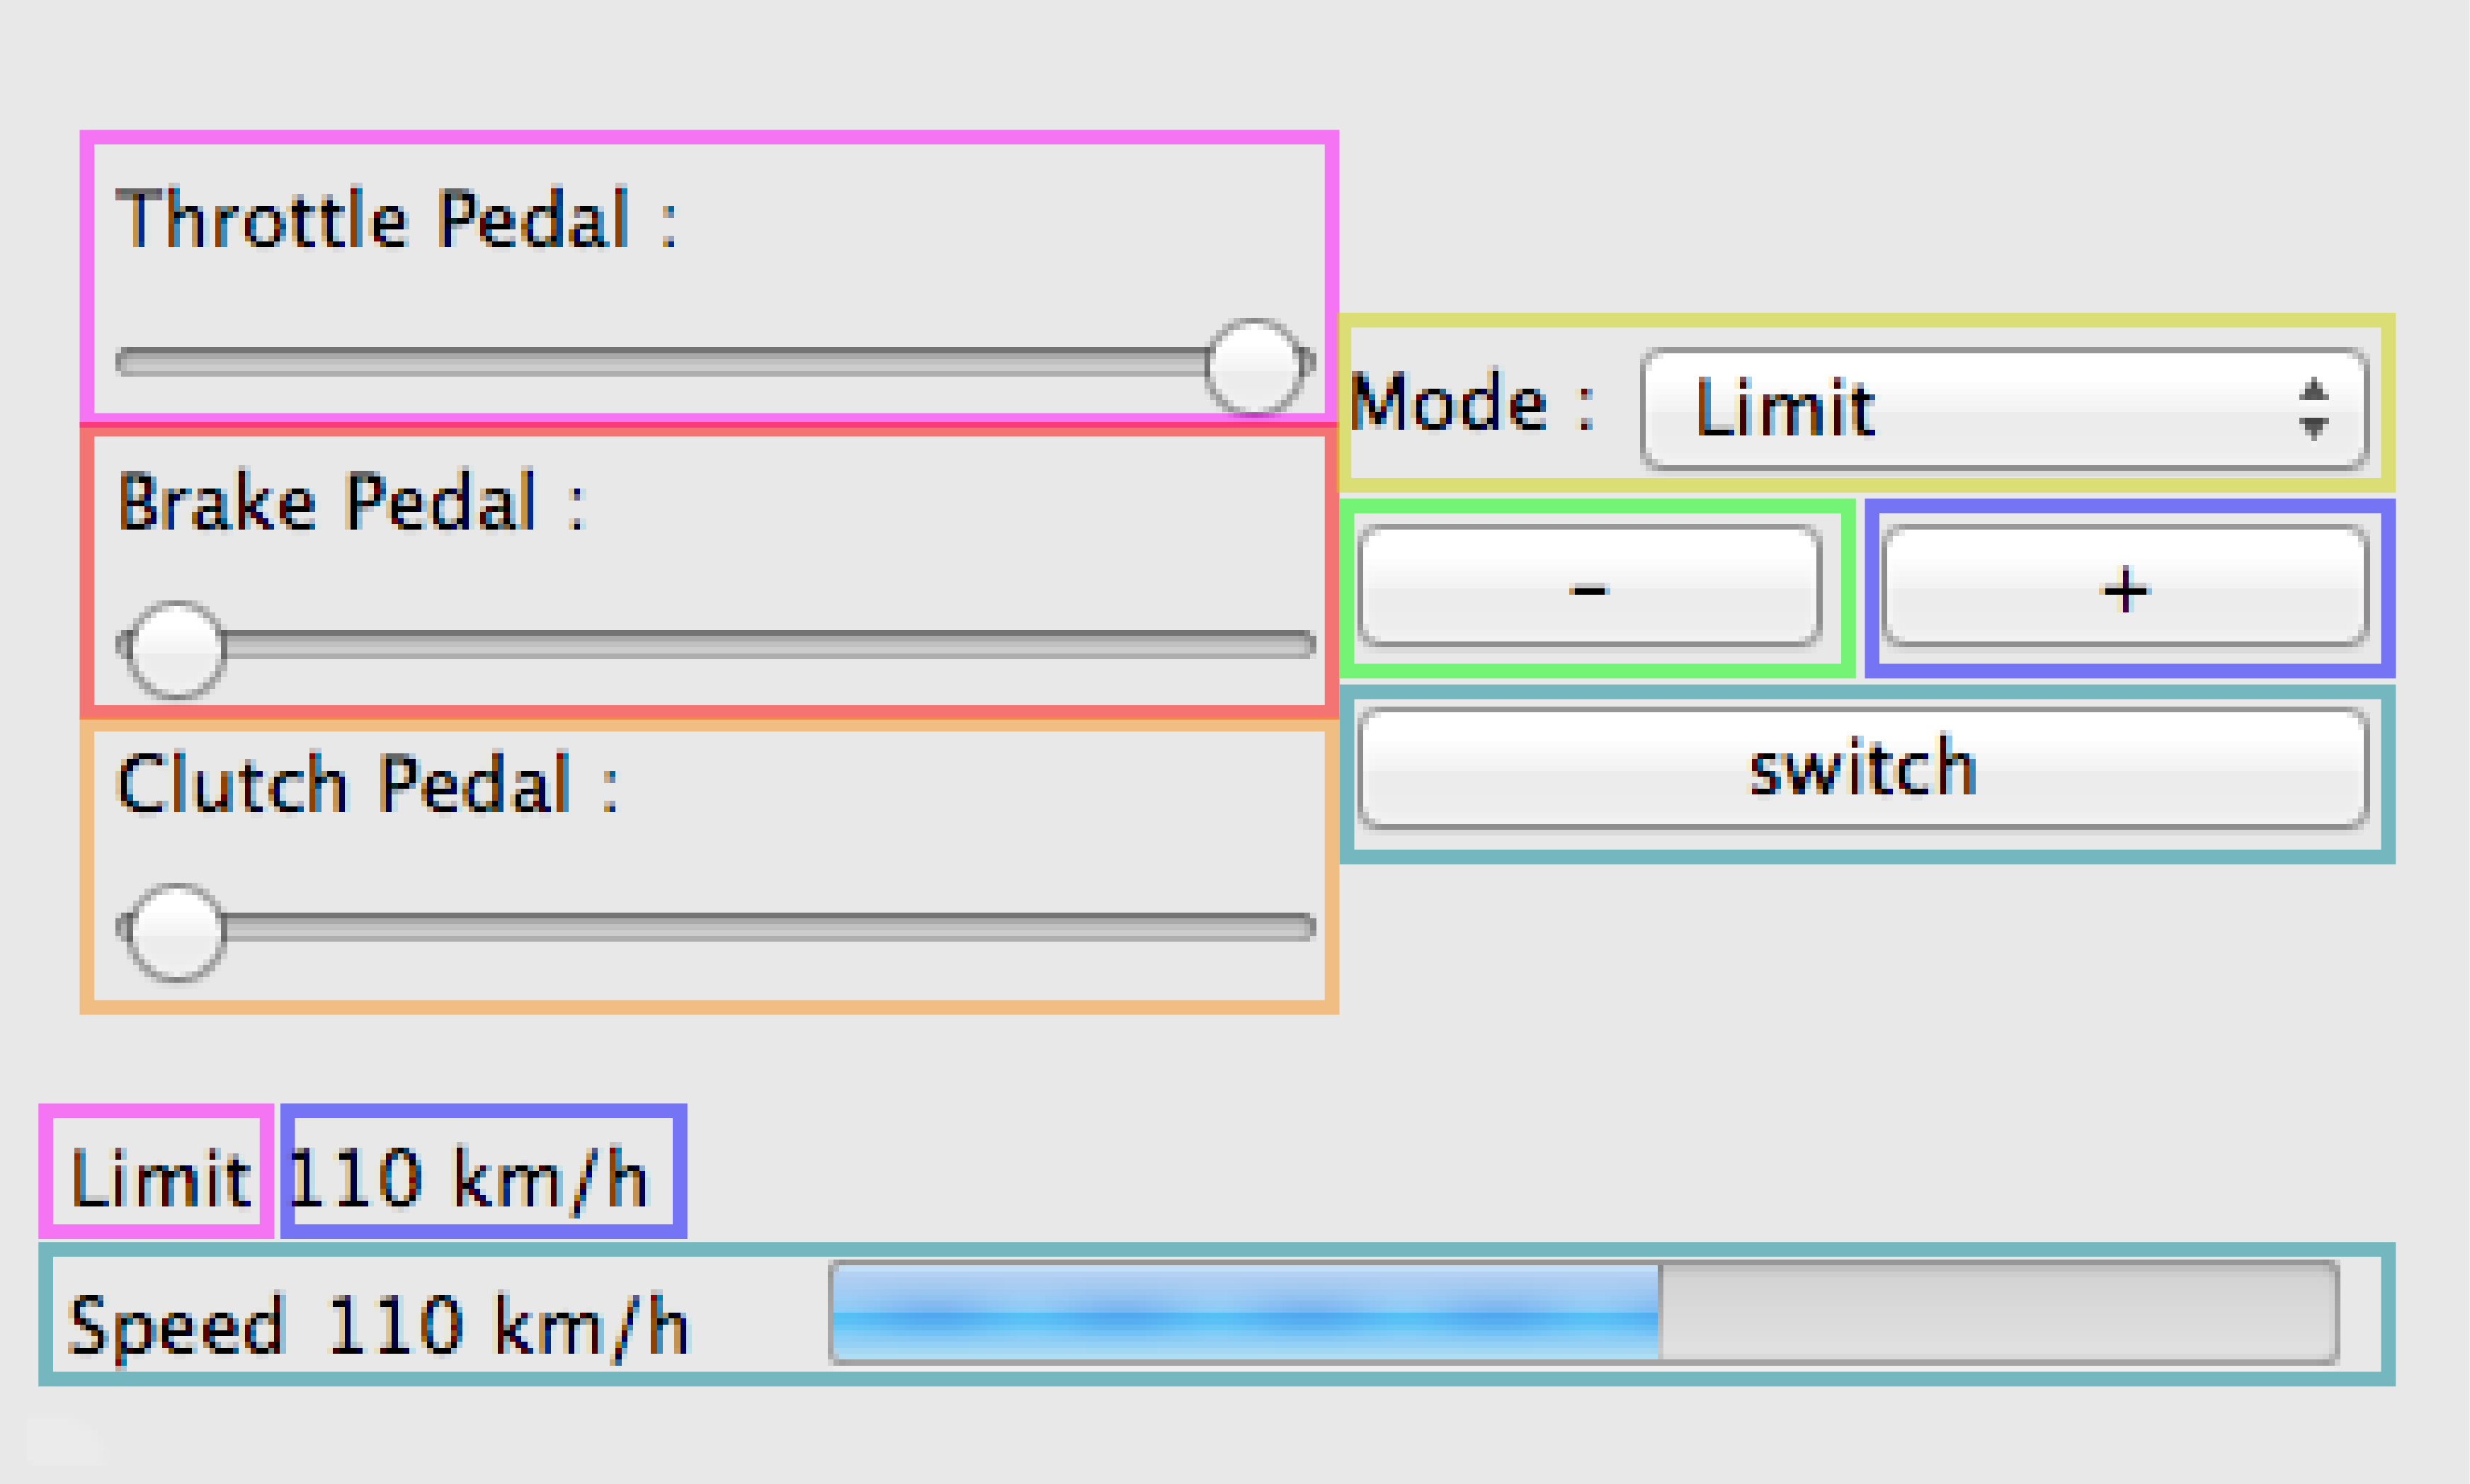
\includegraphics[width=\columnwidth]{screenshothighlighted.png}
\caption{A WIMP concretization of the example application..}
\label{fig:screenshot}
\end{center}
\end{figure}


\begin{figure*}[htbp]
\begin{center}
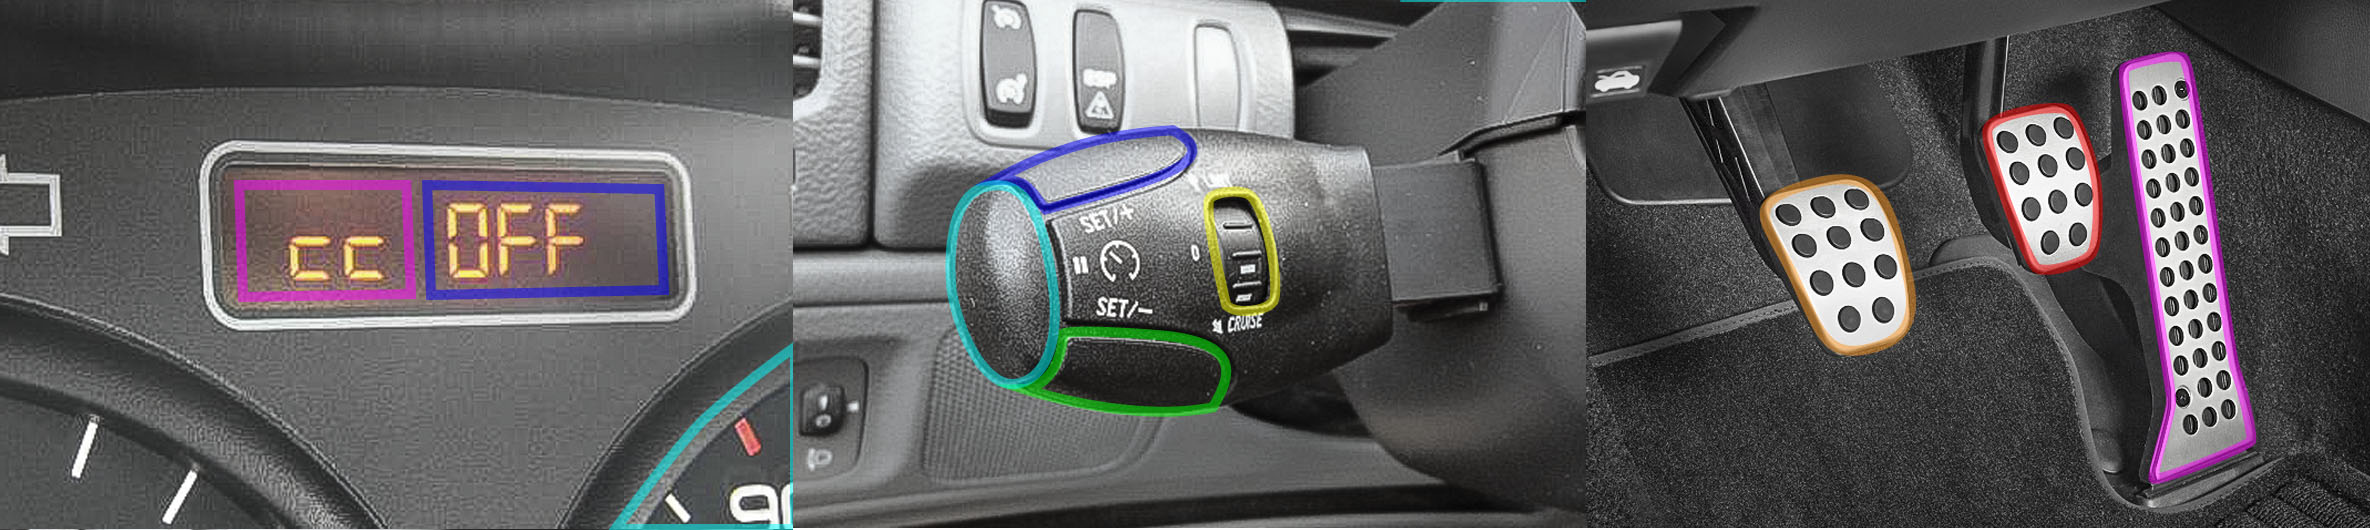
\includegraphics[width=\textwidth]{screenshothighlightedhoriz.jpg}
\caption{The final UI of the example application}
\label{fig:actualcontrols}
\end{center}
\end{figure*}


\begin{minipage}{\columnwidth}
\begin{lstlisting}[caption=LIL code of the example application, label=lilcode]
mode data:
    symbol in {"Off","Limit","Control"}

speedController interactor:
    driver : human actor
    car : system actor

    step : number constant
    minTarget : number constant
    maxTarget : number constant
    
    @mtopLine@m : text or number flow to driver
    @mtopLine@m = if modeCar == "Off" then "" else modeCar
    
    @bbottomLine@b : text or number flow to driver
    @bbottomLine@b = if modeCar == "Off" then "" else targetSpeed
    
    targetSpeed : number flow to car
    @cactualSpeed@c : number flow from car to driver

    @bincrement@b : void event from driver
    on @bincrement@b : targetSpeed = targetSpeed + step
                    toggle = true
                    
    @gdecrement@g : void event from driver
    on @gdecrement@g : targetSpeed = targetSpeed - step
                    toggle = true
  
    @cswitch@c : void event from driver
    on @cswitch@c : toggle = !toggle
    
    toggle : boolean flow
    toggle = clutch < 0.01 && brake < 0.01 && toggle && modeDriver!="Off" 

    @ymodeDriver@y : mode flow from driver

    modeCar : mode flow to car
    modeCar = if toggle then @ymodeDriver@y else "Off"

    @mthrottle@m : number flow from driver
    @rbrake@r : number flow from driver
    @oclutch@o : number flow from driver
    
    @btargetSpeed@b = crop(minTarget,maxTarget,if toggle then targetSpeed else round(@cactualSpeed@c,step)) 
    \end{lstlisting}
\end{minipage}



%    alert : boolean flow to driver
%    alert = actualSpeed > targetSpeed && modeCar!="Off" 


% Balancing columns in a ref list is a bit of a pain because you
% either use a hack like flushend or balance, or manually insert
% a column break.  http://www.tex.ac.uk/cgi-bin/texfaq2html?label=balance
% multicols doesn't work because we're already in two-column mode,
% and flushend isn't awesome, so I choose balance.  See this
% for more info: http://cs.brown.edu/system/software/latex/doc/balance.pdf
%
% Note that in a perfect world balance wants to be in the first
% column of the last page.
%
% If balance doesn't work for you, you can remove that and
% hard-code a column break into the bbl file right before you
% submit:
%
% http://stackoverflow.com/questions/2149854/how-to-manually-equalize-columns-
% in-an-ieee-paper-if-using-bibtex
%
% Or, just remove \balance and give up on balancing the last page.
%
\balance

\bibliographystyle{acm-sigchi}
\bibliography{../bibliography}
\end{document}
